% mnras_template.tex 
%
% LaTeX template for creating an MNRAS paper
%
% v3.0 released 14 May 2015
% (version numbers match those of mnras.cls)
%
% Copyright (C) Royal Astronomical Society 2015
% Authors:
% Keith T. Smith (Royal Astronomical Society)

% Change log
%
% v3.2 July 2023
%	Updated guidance on use of amssymb package
% v3.0 May 2015
%    Renamed to match the new package name
%    Version number matches mnras.cls
%    A few minor tweaks to wording
% v1.0 September 2013
%    Beta testing only - never publicly released
%    First version: a simple (ish) template for creating an MNRAS paper

%%%%%%%%%%%%%%%%%%%%%%%%%%%%%%%%%%%%%%%%%%%%%%%%%%
% Basic setup. Most papers should leave these options alone.
\documentclass[fleqn,usenatbib]{mnras}

% MNRAS is set in Times font. If you don't have this installed (most LaTeX
% installations will be fine) or prefer the old Computer Modern fonts, comment
% out the following line

%\usepackage{newtxtext,newtxmath}
% Depending on your LaTeX fonts installation, you might get better results with one of these:
%\usepackage{mathptmx}
%\usepackage{txfonts}
% Use vector fonts, so it zooms properly in on-screen viewing software
% Don't change these lines unless you know what you are doing
\usepackage[T1]{fontenc}

% Allow "Thomas van Noord" and "Simon de Laguarde" and alike to be sorted by "N" and "L" etc. in the bibliography.
% Write the name in the bibliography as "\VAN{Noord}{Van}{van} Noord, Thomas"
\DeclareRobustCommand{\VAN}[3]{#2}
\let\VANthebibliography\thebibliography
\def\thebibliography{\DeclareRobustCommand{\VAN}[3]{##3}\VANthebibliography}


%%%%% AUTHORS - PLACE YOUR OWN PACKAGES HERE %%%%%

% Only include extra packages if you really need them. Avoid using amssymb if newtxmath is enabled, as these packages can cause conflicts. newtxmatch covers the same math symbols while producing a consistent Times New Roman font. Common packages are:
\usepackage{graphicx}	% Including figure files
\usepackage{amsmath}	% Advanced maths commands

%%%%%%%%%%%%%%%%%%%%%%%%%%%%%%%%%%%%%%%%%%%%%%%%%%

%%%%% AUTHORS - PLACE YOUR OWN COMMANDS HERE %%%%%

% Please keep new commands to a minimum, and use \newcommand not \def to avoid
% overwriting existing commands. Example:
%\newcommand{\pcm}{\,cm$^{-2}$}	% per cm-squared

%%%%%%%%%%%%%%%%%%%%%%%%%%%%%%%%%%%%%%%%%%%%%%%%%%

%%%%%%%%%%%%%%%%%%% TITLE PAGE %%%%%%%%%%%%%%%%%%%

% Title of the paper, and the short title which is used in the headers.
% Keep the title short and informative.
\title[1 homework LLL]{Homework LLL}

% The list of authors, and the short list which is used in the headers.
% If you need two or more lines of authors, add an extra line using \newauthor
\author[Mary Verdugo]{
Mary Verdugo,$^{1}$\thanks{E-mail: mary.verdugo@userena.cl}
\\
% List of institutions
$^{1}$Estudiante de Magister en Astronomia, Universidad de La Serena\\
}

% These dates will be filled out by the publisher
\date{Mon, Nov 27}

% Enter the current year, for the copyright statements etc.
\pubyear{2023}

% Don't change these lines
\begin{document}
\label{firstpage}
\pagerange{\pageref{firstpage}--\pageref{lastpage}}
\maketitle

% Abstract of the paper


% Select between one and six entries from the list of approved keywords.
% Don't make up new ones.


%%%%%%%%%%%%%%%%%%%%%%%%%%%%%%%%%%%%%%%%%%%%%%%% %%

%%%%%%%%%%%%%%%%% BODY OF PAPER %%%%%%%%%%%%%%%%%%

\section{Spectral classification}

Follow the methods obtains from \citet[]{Balogh} with the data from
\citet[]{Dressler}, the aim of this essay is replicate the same figures
9 and 11 from the first paper mentioned with the data of the second, to understand how 
the classification of Balogh is better in fuction to separete between star forming and passive galaxies.
\\
\section{Method}
One of the first thing that we do to understand the comparison is to compare the meta-data of the data with the aim to homogenize the tables.
\\ 
In the case of \citet{Dressler} we have that \textit{the EW of the $H\delta$  is negative when the line present \textbf{emission}} (see figure \ref{dresslertable}). In comparison, the description about this two line features in \citet{Balogh} is: \textit{... When the EW $[OIII]$ index is positive the line is in emission, while the EW $H\delta$ index is positive when the line is in \textbf{absorption}.}
\\
This implies that the data for $H\delta$ from the \citet{Dressler} catalogue, need to be multiplied by $-1$ to homogenize the data. Doing that, we replicate the fig. 9 and fig. 11 from the paper of \citet{Balogh} (see figure \ref{figsbaloghs})

\begin{figure}
	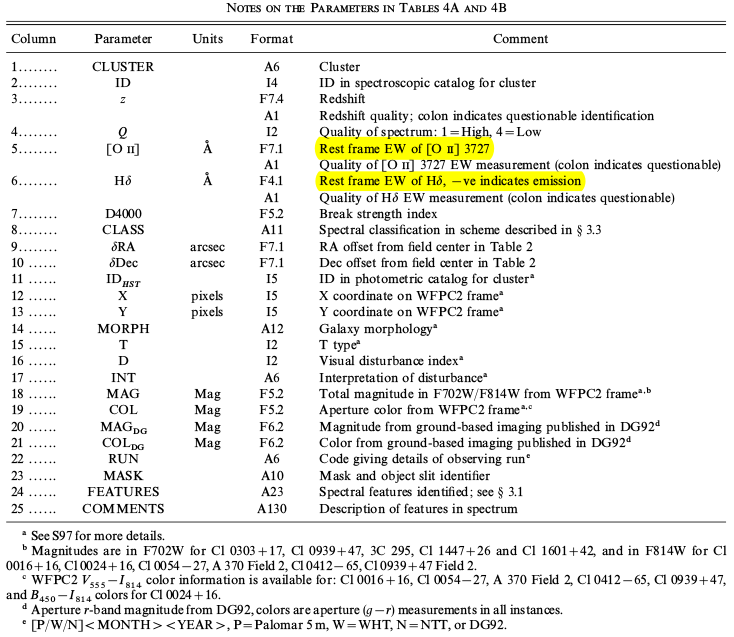
\includegraphics[width=\columnwidth]{/home/patito/Documents/egdatos/tableparameters.png}
    \caption{Capture of the table 5 from \citet{Dressler}}
    \label{dresslertable}
\end{figure}

\begin{figure}
	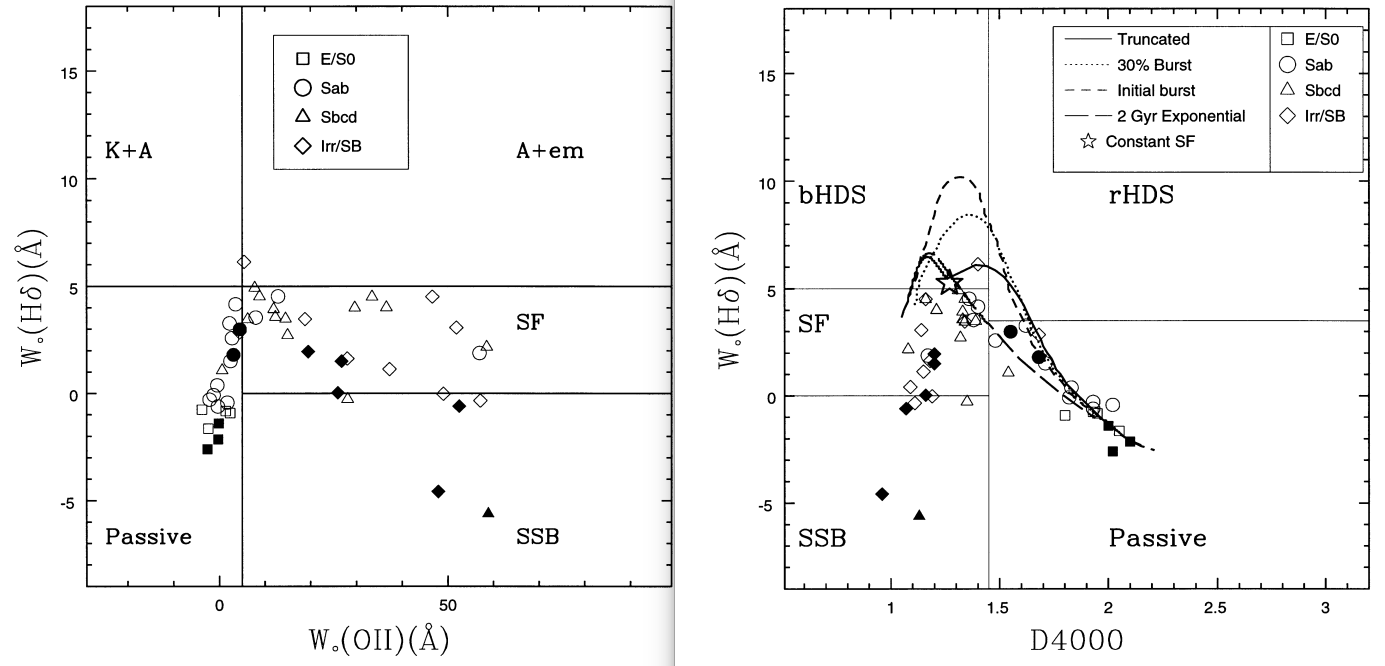
\includegraphics[width=\columnwidth]{/home/patito/Documents/egdatos/pdf/mnrastemplate/imagecomparison.png}
    \caption{figures 9 and 11 from the paper of \citet{Balogh}}
    \label{figsbaloghs}
\end{figure}

\begin{figure}
	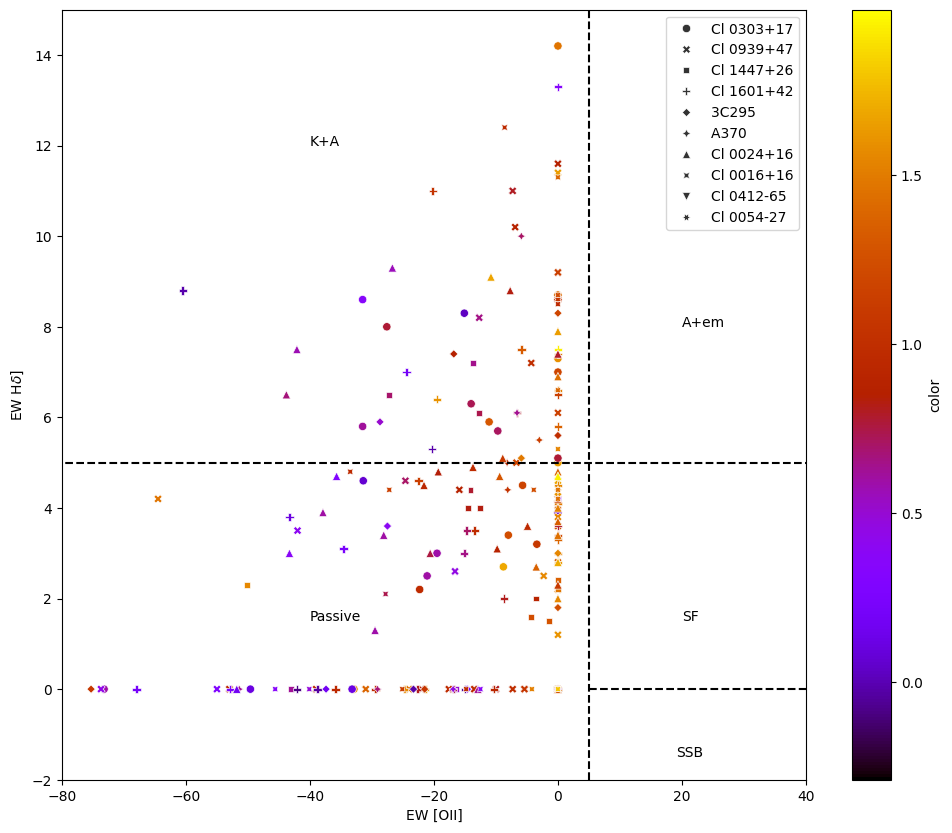
\includegraphics[width=\columnwidth]{//home/patito/Documents/egdatos/pdf/mnrastemplate/plotmio1.png}
	\caption{Figure made to replicate the first panel of the figure \ref{figsbaloghs}, this show the relation between the EW of $O[III]$ and EW of $H\delta$}
\end{figure}




Using a \texttt{python} libraries, we made the sames figures (see figure \ref{plotmio1} and figure \ref{plotmio2})


\section{Conclusions}

The last numbered section should briefly summarise what has been done, and describe
the final conclusions which the authors draw from their work.

\section*{Acknowledgements}

The Acknowledgements section is not numbered. Here you can thank helpful
colleagues, acknowledge funding agencies, telescopes and facilities used etc.
Try to keep it short.

%%%%%%%%%%%%%%%%%%%%%%%%%%%%%%%%%%%%%%%%%%%%%%%%%%
\section*{Data Availability}

 
The inclusion of a Data Availability Statement is a requirement for articles published in MNRAS. Data Availability Statements provide a standardised format for readers to understand the availability of data underlying the research results described in the article. The statement may refer to original data generated in the course of the study or to third-party data analysed in the article. The statement should describe and provide means of access, where possible, by linking to the data or providing the required accession numbers for the relevant databases or DOIs.




%%%%%%%%%%%%%%%%%%%% REFERENCES %%%%%%%%%%%%%%%%%%

% The best way to enter references is to use BibTeX:

\bibliographystyle{mnras}
\bibliography{example} % if your bibtex file is called example.bib


% Alternatively you could enter them by hand, like this:
% This method is tedious and prone to error if you have lots of references
%\begin{thebibliography}{99}
%\bibitem[\protect\citeauthoryear{Author}{2012}]{Author2012}
%Author A.~N., 2013, Journal of Improbable Astronomy, 1, 1
%\bibitem[\protect\citeauthoryear{Others}{2013}]{Others2013}
%Others S., 2012, Journal of Interesting Stuff, 17, 198
%\end{thebibliography}

%%%%%%%%%%%%%%%%%%%%%%%%%%%%%%%%%%%%%%%%%%%%%%%%%%

%%%%%%%%%%%%%%%%% APPENDICES %%%%%%%%%%%%%%%%%%%%%

\appendix

\section{Some extra material}

If you want to present additional material which would interrupt the flow of the main paper,
it can be placed in an Appendix which appears after the list of references.

%%%%%%%%%%%%%%%%%%%%%%%%%%%%%%%%%%%%%%%%%%%%%%%%%%


% Don't change these lines
\bsp	% typesetting comment
\label{lastpage}
\end{document}

% End of mnras_template.tex
